% ==================================================
% 第三章　研究方法與全身模型預測控制器設計
% ==================================================
\chapter{研究方法與全身模型預測控制器設計}
\label{c:methodology}
\label{c:Mathodology}

本章以 Tang 等人\cite{tang2024gmpc}之幾何模型預測控制為基礎，
結合手臂設定點追蹤、動態障礙預測與操作參考，
在共同時間基準下求解底盤速度及手臂設定點變化率。
以下說明全身運動學、增廣模型、控制問題、視覺操作及執行整合。

% ==================================================
% 3.1 底盤幾何運動與全身運動學
% ==================================================
\section{底盤幾何運動與全身運動學}
\label{sec:wholebody_kinematics}

末端位姿同時受底盤與手臂構型影響。
本節以平面剛體描述底盤運動，再嵌入三維運動鏈，
建立預測模型與末端追蹤所需的幾何關係。

% ==================================================
% 3.1.1 座標系定義與位姿表示
% ==================================================
\subsection{座標系定義與位姿表示}
\label{subsec:frames_pose_representation}

定義世界、底盤、手臂基座及工具中心點座標系，
分別記為 $\mathcal F_W$、$\mathcal F_B$、$\mathcal F_A$ 與 $\mathcal F_E$。
底盤座標對應 \texttt{base\_footprint}，
$x_B$ 向前、$y_B$ 向左、$z_B$ 向上。
以 $ {}^iT_j$ 表示由座標系 $j$ 轉換至 $i$ 的齊次變換。
底盤位姿與手臂關節角為
\begin{equation}
    X_B=
    \begin{bmatrix}
        R_B(\theta_B)&p_B\\
        \mathbf 0_{1\times2}&1
    \end{bmatrix}\in\mathrm{SE}(2),
    \qquad
    p_B=\begin{bmatrix}x_B&y_B\end{bmatrix}^{\top},
    \quad q_a\in\mathbb R^6 .
    \label{eq:ch3_base_pose}
\end{equation}
其中 $R_B$ 為平面旋轉矩陣。
指數與對數映射的定義依 Sol\`a 等人\cite{sola2018micro}之整理。
如\cref{fig:ref_rotation_representation}所示，
角度主值跨越邊界時會跳變，對應旋轉仍可連續表示。

世界座標用於導航與操作目標，底盤座標用於速度命令及持物構型。
對數映射提供局部誤差座標，其使用須配合旋轉分支與參考位姿。

\begin{figure}[htbp]
    \centering
    \includegraphics[width=0.88\textwidth]{figsrc/ch03/rotation_representation_redrawn.png}
    \caption{旋轉與角度主值表示之比較：
    (a) 旋轉方向連續通過角度邊界；
    (b) 對應角度主值產生包絡跳變。}
    \label{fig:ref_rotation_representation}
\end{figure}

% ==================================================
% 3.1.2 底盤 SE(2) 運動模型與追蹤誤差
% ==================================================
\subsection{底盤 SE(2) 運動模型與追蹤誤差}
\label{subsec:base_se2_model_error}

全向底盤的本體速度為
$\xi_B=[v_x^B,v_y^B,\omega_B]^{\top}$，
滿足 $\dot X_B=X_B\widehat{\xi}_B$。
令參考位姿為 $X_r$，其本體速度為 $\xi_r$，
定義幾何追蹤誤差及速度偏差為
\begin{equation}
    E_B=X_r^{-1}X_B,\qquad
    e_B=(\log E_B)^\vee,\qquad
    \delta\xi=\xi_B-\xi_r .
    \label{eq:ch3_geometric_tracking_error}
\end{equation}
其中 $(\widehat{\cdot})$ 與 $(\cdot)^\vee$ 為速度向量及李代數矩陣間的映射。
由相對變換的微分，在小誤差下建立局部模型，
並以前向歐拉法離散化：
\begin{equation}
    e_{B,k+1}=A_{B,k}e_{B,k}+\Delta t\,\delta\xi_k,
    \qquad
    A_{B,k}=I_3-\Delta t\,\operatorname{ad}(\xi_{r,k}).
    \label{eq:ch3_discrete_base_error_model}
\end{equation}
此處 $\operatorname{ad}(\xi)\eta=
([\widehat\xi,\widehat\eta])^\vee$，
$[A,B]=AB-BA$。
控制器每次更新均由目前位姿重新計算誤差，
其近似精度取決於追蹤偏差、控制週期及預測時域。

% ==================================================
% 3.1.3 移動機械臂正向運動學與全身雅可比矩陣
% ==================================================
\subsection{移動機械臂正向運動學與全身雅可比矩陣}
\label{subsec:wholebody_fk_jacobian}

將 $X_B$ 嵌入三維變換 $ {}^WT_B$，平移為 $[x_B,y_B,0]^\top$。
手臂安裝變換 $ {}^BT_A$ 的平移為 $(0.11,0,0.33)$ m，
包含底盤高度與安裝偏移。末端世界位姿為
\begin{equation}
    {}^WT_E={}^WT_B\,{}^BT_A\,{}^AT_E(q_a).
    \label{eq:ch3_wholebody_forward_kinematics}
\end{equation}
$ {}^AT_E$ 包含工具中心點（Tool Center Point, TCP）偏移。
末端線速度與角速度均表示於世界座標：
\begin{equation}
    {}^W\nu_E=
    \begin{bmatrix}{}^W\dot p_E\\{}^W\omega_E\end{bmatrix}
    =
    \begin{bmatrix}{}^WJ_B&{}^WJ_A\end{bmatrix}
    \begin{bmatrix}\xi_B\\\dot q_a\end{bmatrix}.
    \label{eq:ch3_wholebody_geometric_velocity}
\end{equation}
令 $r_{BE}={}^Wp_E-{}^Wp_B$，其中 $ {}^Wp_B=[x_B,y_B,0]^\top$，
底盤雅可比為
\begin{equation}
    {}^WJ_B=
    \begin{bmatrix}
        \cos\theta_B&-\sin\theta_B&-(r_{BE})_y\\
        \sin\theta_B& \cos\theta_B& (r_{BE})_x\\
        0&0&0\\
        0&0&0\\
        0&0&0\\
        0&0&1
    \end{bmatrix}.
    \label{eq:ch3_base_geometric_jacobian}
\end{equation}
第三欄包含偏航造成的 TCP 線速度與角速度。
以世界構型變化率為輸入時，對應區塊為
$J_{\chi,B}={}^WJ_B\operatorname{diag}(R_B^\top,1)$，
$J_{\chi,A}={}^WJ_A$。
底盤與手臂的共同作用如\cref{fig:ch3_wholebody_motion_coupling}所示。
以下以 $\chi=[x_B,y_B,\theta_B,q_a^\top]^\top$ 表示九維全身構型；
實際關節速度 $\dot q_a$ 與控制輸出的設定點變化率分別處理。

\begin{figure}[htbp]
    \centering
    \includegraphics[width=0.98\textwidth]{figsrc/ch03/wholebody_motion_coupling.png}
    \caption{底盤側移時之全身運動學耦合：
    (a) 底盤移動前；(b) 底盤側移後，手臂調整構型以維持相同末端目標。}
    \label{fig:ch3_wholebody_motion_coupling}
\end{figure}

% ==================================================
% 3.2 手臂設定點追蹤與增廣預測模型
% ==================================================
\section{手臂設定點追蹤與增廣預測模型}
\label{sec:arm_augmented_prediction}

手臂位置介面包含設定點積分與伺服追蹤。
本節將實際關節位置與設定點納入狀態，
再與底盤幾何誤差組合，描述命令至構型的響應。

% ==================================================
% 3.2.1 手臂位置命令與伺服追蹤動態
% ==================================================
\subsection{手臂位置命令與伺服追蹤動態}
\label{subsec:arm_setpoint_servo}

令 $u_a$ 為設定點變化率、$s_a$ 為位置設定點。
依命令執行特性\cite{grandia2019frequency}，
以物理步長 $\Delta t_p$ 建立逐軸一階仿射模型：
\begin{equation}
    \begin{aligned}
        q_a^{j+1}&=(I_6-D_\alpha)q_a^j+D_\alpha s_a^j+b_a,\\
        s_a^{j+1}&=s_a^j+\Delta t_p u_a^j .
    \end{aligned}
    \label{eq:ch3_physics_step_arm_model}
\end{equation}
其中 $D_\alpha=\operatorname{diag}(\alpha_1,\ldots,\alpha_6)$，
$0<\alpha_i<1$，$b_a$ 為每步偏置。
$s_a^j$ 是作用於第 $j$ 至 $j+1$ 步的設定點。
固定設定點下的穩態偏移為 $D_\alpha^{-1}b_a$，
且 $u_a=0$ 時關節仍可能持續追蹤，因此 $u_a$ 不等同 $\dot q_a$。

% ==================================================
% 3.2.2 實際關節位置與設定點之增廣狀態
% ==================================================
\subsection{實際關節位置與設定點之增廣狀態}
\label{subsec:augmented_arm_state}

令控制週期 $\Delta t=m\Delta t_p$。
在一個控制週期內保持 $u_a$ 固定，
將物理步模型合成 $m$ 次，得到
\begin{equation}
    \begin{aligned}
        q_{a,k+1}&=A_q q_{a,k}+A_s s_{a,k}+B_a u_{a,k}+c_a,\\
        s_{a,k+1}&=s_{a,k}+\Delta t u_{a,k}.
    \end{aligned}
    \label{eq:ch3_control_step_arm_model}
\end{equation}
令 $\beta_i=1-\alpha_i$，
則 $A_q=\operatorname{diag}(\beta_i^m)$、$A_s=I_6-A_q$，
$B_a$ 的第 $i$ 個對角元素為
$\alpha_i\Delta t_p\sum_{\ell=0}^{m-1}\ell\beta_i^{m-1-\ell}$，
且 $(c_a)_i=(b_a)_i(1-\beta_i^m)/\alpha_i$。

結合底盤誤差，定義增廣狀態與控制輸入為
\[
    \begin{aligned}
        \zeta_k&=[e_{B,k}^\top,q_{a,k}^\top,s_{a,k}^\top]^\top\in\mathbb R^{15},\\
        u_k&=[\delta\xi_k^\top,u_{a,k}^\top]^\top\in\mathbb R^9 .
    \end{aligned}
\]
則增廣預測模型為
\begin{equation}
    \begin{gathered}
    \zeta_{k+1}=F_k\zeta_k+G_ku_k+d_k,\\
    F_k=
    \begin{bmatrix}
        A_{B,k}&0&0\\
        0&A_q&A_s\\
        0&0&I_6
    \end{bmatrix},
    \quad
    G_k=
    \begin{bmatrix}
        \Delta t I_3&0\\
        0&B_a\\
        0&\Delta t I_6
    \end{bmatrix}.
    \end{gathered}
    \label{eq:ch3_augmented_prediction_dynamics}
\end{equation}
其中 $d_k=[0_3^\top,c_a^\top,0_6^\top]^\top$。
此為底盤命令於控制拍內保持固定的基本形式；
採拍內斜坡的階段另依第 3.7.1 節修正底盤預測。
末端位姿由 $X_B=X_r\exp(\widehat e_B)$ 與預測的實際關節位置重建，
使分塊狀態轉移仍可透過共同末端目標耦合。
設定點與實際位置之差異如\cref{fig:ch3_arm_setpoint_tracking}所示。

\begin{figure}[htbp]
    \centering
    \includegraphics[width=0.98\textwidth]{figsrc/ch03/arm_setpoint_tracking.png}
    \caption{設定點與實際關節位置之追蹤關係：
    (a) 設定點固定；(b) 關節持續追蹤；(c) 關節逐漸接近設定點。
    虛線與實線分別表示位置設定點與實際關節位置。}
    \label{fig:ch3_arm_setpoint_tracking}
\end{figure}

% ==================================================
% 3.2.3 多步預測模型建立與參數辨識
% ==================================================
\subsection{多步預測模型建立與參數辨識}
\label{subsec:multistep_prediction_identification}

令 $i|k$ 表示第 $k$ 個控制週期對未來第 $i$ 步的預測。
初始設定點採執行端回報值，以保留尚未完成的追蹤運動。
堆疊 $N$ 步狀態與輸入為
$\mathbf Z_k=[\zeta_{1|k}^\top,\ldots,\zeta_{N|k}^\top]^\top$、
$\mathbf U_k=[u_{0|k}^\top,\ldots,u_{N-1|k}^\top]^\top$，則
\begin{equation}
    \mathbf Z_k=\Phi_k\zeta_{0|k}+\Gamma_k\mathbf U_k+\eta_k .
    \label{eq:ch3_condensed_augmented_prediction}
\end{equation}
$\Phi_k$、$\Gamma_k$ 與 $\eta_k$ 分別描述初始狀態、控制序列與累積偏置的影響。
對第 $r$ 軸，令 $\Delta q_r^j=q_r^{j+1}-q_r^j$、
$\epsilon_r^j=s_r^j-q_r^j$，依命令實際作用區間對齊量測後辨識：
\begin{equation}
    (\hat\alpha_r,\hat b_r)=
    \underset{\alpha_r,b_r}{\operatorname{arg\,min}}
    \sum_{j\in\mathcal I_{\mathrm{est}}}
    \left(\Delta q_r^j-\alpha_r\epsilon_r^j-b_r\right)^2.
    \label{eq:ch3_arm_parameter_identification}
\end{equation}
$\mathcal I_{\mathrm{est}}$ 為估計資料索引，估計後檢查 $0<\hat\alpha_r<1$，
並以時間分離資料驗證單步與多步誤差。
多步結果須區分使用後續實錄設定點的條件重播，
以及只依起始狀態與當時可用命令推進的預測。

% ==================================================
% 3.3 全身預測控制之目標函數與限制條件
% ==================================================
\section{全身預測控制之目標函數與限制條件}
\label{sec:wholebody_objective_constraints}

控制問題整合底盤路徑與末端目標，
並以命令、關節及輪級限制決定兩者的運動分配。

% ==================================================
% 3.3.1 底盤與末端位姿追蹤目標
% ==================================================
\subsection{底盤與末端位姿追蹤目標}
\label{subsec:wholebody_tracking_objective}

令 $\|x\|_Q^2=x^\top Qx$，末端目標與預測位姿均以世界座標表示。
六維殘差定義為
\begin{equation}
    r_{E,i|k}=
    \begin{bmatrix}
        p_{E,i|k}^{d}-p_{E,i|k}\\
        R_{E,i|k}
        [\log(R_{E,i|k}^{\top}R_{E,i|k}^{d})]^\vee
    \end{bmatrix}.
    \label{eq:ch3_tcp_pose_residual}
\end{equation}
姿態殘差轉至世界座標，與幾何雅可比一致。完整成本包含六項：
\begin{equation}
    J_{\mathrm{total}}
    =J_B+J_E+J_u+J_\Delta+J_{\mathrm{post}}+J_\varepsilon .
    \label{eq:ch3_wholebody_objective}
\end{equation}
其中前四項為基本成本，構型引導與避障鬆弛依任務啟用。
令完整命令 $v=[\xi_B^\top,u_a^\top]^\top$，$\xi_B=\xi_r+\delta\xi$；
以下以非負對角權重展開各項。

\noindent\textbf{（一）底盤追蹤成本。}
令底盤誤差向量與對角權重矩陣分別為
\[
    \begin{aligned}
        e_B&=[e_{B,x},e_{B,y},e_{B,\theta}]^\top,\\
        Q_{B,i}&=\operatorname{diag}
        (w_{B,x,i},w_{B,y,i},w_{B,\theta,i}).
    \end{aligned}
\]
則底盤追蹤成本為
\begin{equation}
    J_B=\sum_{i=1}^{N}\left[
        w_{B,x,i}e_{B,x,i|k}^{2}
        +w_{B,y,i}e_{B,y,i|k}^{2}
        +w_{B,\theta,i}e_{B,\theta,i|k}^{2}\right].
    \label{eq:ch3_base_tracking_cost_expanded}
\end{equation}
前兩項懲罰相對路徑的位置偏差，第三項懲罰朝向偏差；
其誤差分量依式\eqref{eq:ch3_geometric_tracking_error}的位姿對數定義。
調大對應權重，會提高該方向追蹤誤差在最佳化中的代價。
$Q_{B,N}$ 是預測最後一步使用的終端權重，
用於調整時域末端的底盤追蹤要求，已包含於上述第 $N$ 項。

\noindent\textbf{（二）末端位姿追蹤成本。}
將六維殘差分為位置向量 $r_{p,i|k}$ 與姿態向量 $r_{R,i|k}$，
使 $r_{E,i|k}=[r_{p,i|k}^\top,r_{R,i|k}^\top]^\top$。
目前三個位置方向共用權重 $w_p$，三個姿態方向共用權重 $w_R$，
即 $W_E=\operatorname{diag}(w_p I_3,w_R I_3)$，可展開為
\begin{equation}
    \begin{aligned}
        J_E=\sum_{i=1}^{N}\big[&
        w_p(r_{p,x,i|k}^{2}+r_{p,y,i|k}^{2}+r_{p,z,i|k}^{2})\\
        &+w_R(r_{R,x,i|k}^{2}+r_{R,y,i|k}^{2}+r_{R,z,i|k}^{2})\big].
    \end{aligned}
    \label{eq:ch3_tcp_tracking_cost_expanded}
\end{equation}
位置項要求 TCP 接近目標，姿態項要求工具方向符合操作需求，兩者分別以公尺與弧度計算。
權重依容許偏差設定相對尺度；此項透過末端運動學共同調整底盤與手臂。
持物階段改用第 3.6.3 節的底盤相對殘差。

\noindent\textbf{（三）輸入大小成本。}
以 $\delta\xi=[\delta v_x^B,\delta v_y^B,\delta\omega_B]^\top$ 表示底盤速度修正量，
令 $R=\operatorname{diag}(r_x,r_y,r_\omega,r_{a,1},\ldots,r_{a,6})$，則
\begin{equation}
    \begin{aligned}
        J_u=\sum_{i=0}^{N-1}\big[&
        r_x(\delta v_{x,i|k}^{B})^{2}
        +r_y(\delta v_{y,i|k}^{B})^{2}
        +r_\omega(\delta\omega_{B,i|k})^{2}\\
        &+\sum_{j=1}^{6}r_{a,j}u_{a,j,i|k}^{2}\big].
    \end{aligned}
    \label{eq:ch3_input_cost_expanded}
\end{equation}
底盤部分抑制過大的速度修正；修正量為零時，底盤仍可沿非零參考速度行進。
手臂部分抑制設定點變化率，實際關節運動仍由第 3.2 節的追蹤模型決定。
輸入權重亦提供數值正則化，與關節及速度硬限制共同約束命令。

\noindent\textbf{（四）命令差分成本。}
令 $v_k^{\mathrm{prev}}$ 為預測生效起點前的放行命令，則
\begin{equation}
    \begin{gathered}
        \Delta v_{i|k}=
        \begin{cases}
            v_{0|k}-v_k^{\mathrm{prev}},&i=0,\\
            v_{i|k}-v_{i-1|k},&i=1,\ldots,N-1,
        \end{cases}\\
        \Delta\xi_{B,i|k}=
        (\xi_{r,i|k}-\xi_{r,i-1|k})
        +(\delta\xi_{i|k}-\delta\xi_{i-1|k}),\quad i\geq1 .
    \end{gathered}
    \label{eq:ch3_command_difference_definition}
\end{equation}
若生效時刻尚未到達，$v_k^{\mathrm{prev}}$ 由既定在途排程前推取得。
其中 $\Delta\xi_B=[\Delta v_x^B,\Delta v_y^B,\Delta\omega_B]^\top$，
$\Delta u_a$ 為手臂設定點變化率的差分。
令 $S=\operatorname{diag}(\sigma_x,\sigma_y,\sigma_\omega,
\sigma_{a,1},\ldots,\sigma_{a,6})$，可得
\begin{equation}
    \begin{aligned}
        J_\Delta=\sum_{i=0}^{N-1}\big[&
        \sigma_x(\Delta v_{x,i|k}^{B})^{2}
        +\sigma_y(\Delta v_{y,i|k}^{B})^{2}
        +\sigma_\omega(\Delta\omega_{B,i|k})^{2}\\
        &+\sum_{j=1}^{6}\sigma_{a,j}(\Delta u_{a,j,i|k})^{2}\big].
    \end{aligned}
    \label{eq:ch3_smoothness_cost_expanded}
\end{equation}
此項抑制相鄰完整命令的突變，包含底盤參考速度改變所造成的差分。
調大權重通常使命令較平緩，也可能增加快速追蹤時的落後。
此處採命令差，其與命令變化率的換算為 $\Delta v/\Delta t$；
速度與命令變化的可執行上限另由限制條件施加。

\noindent\textbf{（五）構型引導與（六）避障鬆弛成本。}
啟用構型引導時，以參考關節構型 $q_{a,i}^{\mathrm{exp}}$ 引導手臂分支；
啟用 CBF 鬆弛時，對各限制群組與預測步的鬆弛量加入成本：
\begin{equation}
    \begin{aligned}
        J_{\mathrm{post}}
        &=\sum_{i=1}^{N}\sum_{j=1}^{6}
        \kappa_j(q_{a,j,i|k}-q_{a,j,i}^{\mathrm{exp}})^2,\\
        J_\varepsilon
        &=\sum_{i=0}^{N-1}\sum_{g\in\mathcal C}
        w_{\varepsilon,g,i}\varepsilon_{g,i|k}^{2} .
    \end{aligned}
    \label{eq:ch3_optional_cost_terms}
\end{equation}
$\kappa_j$ 為 $Q_{\mathrm{post}}$ 的對角係數，參考構型依第 3.5.4 節生成；
$\mathcal C$ 為啟用的 CBF 限制群組，$w_{\varepsilon,g,i}>0$ 為鬆弛權重。
鬆弛權重越大，違反屏障條件的代價越高，仍須檢查實際鬆弛量與間距。
未啟用的選用成本取零，關節及速度等硬限制持續施加。

各權重依容許偏差與命令尺度設定，再調整路徑追蹤、操作精度及命令平滑的相對比重。
手臂命令以設定點變化率上限 $\bar u_a$ 正規化，
取 $r_{a,j}=w_a/\bar u_a^2$、$\sigma_{a,j}=w_s/\bar u_a^2$；
$w_a,w_s$ 為調整係數，實際數值與啟用組合於第四章列示。

% ==================================================
% 3.3.2 關節、命令變化與輪級運動限制
% ==================================================
\subsection{關節、命令變化與輪級運動限制}
\label{subsec:joint_command_wheel_constraints}

令 $\mu\in\mathbb R_{\geq0}^6$ 為關節限位餘量，
同時限制實際關節位置、設定點、完整命令與命令變化：
\begin{equation}
    \begin{gathered}
        q_{\min}+\mu\leq q_{a,i|k}\leq q_{\max}-\mu,\qquad
        q_{\min}+\mu\leq s_{a,i|k}\leq q_{\max}-\mu,\\
        v_{\min}\leq v_{i|k}\leq v_{\max},\qquad
        -\Delta v_{\max}\leq\Delta v_{i|k}\leq\Delta v_{\max}.
    \end{gathered}
    \label{eq:ch3_joint_command_limits}
\end{equation}
實際位置與設定點分別約束目前構型及尚待追蹤的命令累積。
依四輪十字配置的輪序與正向約定，
\begin{equation}
    \dot q_w=\frac{1}{r_w}W\xi_B,\qquad
    W=
    \begin{bmatrix}
        0&1&L\\-1&0&L\\0&-1&L\\1&0&L
    \end{bmatrix}.
    \label{eq:ch3_wheel_command_mapping}
\end{equation}
$r_w$ 為輪半徑，$L$ 為車心至輪心距離。
輪速及輪速命令變化率限制為
\begin{equation}
    \left|\frac{W\xi_{B,i|k}}{r_w}\right|\leq\bar\omega_w,\qquad
    \left|\frac{W(\xi_{B,i|k}-\xi_{B,i-1|k})}{r_w}\right|
    \leq\Delta t\,\bar a_w .
    \label{eq:ch3_wheel_speed_acceleration_limits}
\end{equation}
不等式逐分量成立，上限以四維向量表示。
輪級限制描述平移與旋轉共用的致動能力，與各軸速度框共同施加。

% ==================================================
% 3.3.3 最佳化問題建構與數值求解
% ==================================================
\subsection{最佳化問題建構與數值求解}
\label{subsec:wholebody_qp_formulation}

沿名目序列 $\bar{\mathbf U}_k$ 建立末端運動學的一次局部近似。
目前底盤名目速度偏差取零，手臂名目序列依階段採零速或由參考構型反算。
令 $\Gamma_{i,k}$ 為式\eqref{eq:ch3_condensed_augmented_prediction}的第 $i$ 步列區塊，
$C_i=\partial[x_B,y_B,\theta_B]^\top/\partial e_B$
為 $X_B=X_r\exp(\widehat e_B)$ 的局部微分。
末端幾何位移對增廣狀態的映射為
\begin{equation}
    \mathcal J_{E,i}=
    \begin{bmatrix}
        J_{\chi,B,i}C_i&J_{\chi,A,i}&0_{6\times6}
    \end{bmatrix}\in\mathbb R^{6\times15}.
    \label{eq:ch3_tcp_augmented_geometric_jacobian}
\end{equation}
各矩陣在名目預測狀態計算；設定點透過追蹤動態影響未來關節位置。
對小構型變化與小姿態誤差，殘差近似為
\begin{equation}
    \begin{aligned}
        r_{E,i|k}
        &\approx\bar r_{E,i|k}
        -L_{i,k}(\mathbf U_k-\bar{\mathbf U}_k)\\
        &=r_{0,i|k}-L_{i,k}\mathbf U_k,\\
        L_{i,k}&=\mathcal J_{E,i}\Gamma_{i,k},\qquad
        r_{0,i|k}=\bar r_{E,i|k}+L_{i,k}\bar{\mathbf U}_k .
    \end{aligned}
    \label{eq:ch3_tcp_affine_residual}
\end{equation}
$\bar r_{E,i|k}$ 為名目殘差。
$L_{i,k}$ 同時包含底盤與手臂分量，使末端成本產生兩者的交叉項。

將各步追蹤殘差、完整命令差分及構型引導代入式\eqref{eq:ch3_wholebody_objective}，
省略常數項後，累加得到二次項矩陣 $H_k$ 與一次項向量 $g_k$；
避障鬆弛成本另以 $J_\varepsilon$ 表示。
連同命令、關節、輪級與避障限制，形成二次規劃（Quadratic Programming, QP）：
\begin{equation}
    \begin{aligned}
        \min_{\mathbf U_k,\,\varepsilon}\quad&
        \frac12\mathbf U_k^\top H_k\mathbf U_k
        +g_k^\top\mathbf U_k+J_\varepsilon\\
        \text{subject to}\quad&
        A_{\mathrm{ineq},k}\mathbf U_k
        +B_{\varepsilon,k}\varepsilon\leq b_{\mathrm{ineq},k},
        \qquad\varepsilon\geq0 .
    \end{aligned}
    \label{eq:ch3_wholebody_qp}
\end{equation}
$\varepsilon$ 僅放寬允許鬆弛的限制，硬限制對應的 $B_{\varepsilon,k}$ 列為零。
固定局部近似且權重半正定時為凸 QP；輸入權重正定時，基本控制成本嚴格凸。
此性質限於當次近似問題，不代表非線性原問題全域凸。
目前手臂啟用的耦合問題以 Goldfarb--Idnani 方法\cite{goldfarb1983dual}求解，
必要時以 OSQP\cite{stellato2020osqp}備援；純底盤問題使用 OSQP。
候選解均須核對有限性、求解狀態及限制殘差。

% ==================================================
% 3.3.4 滾動時域控制原則
% ==================================================
\subsection{滾動時域控制原則}
\label{subsec:wholebody_receding_horizon}

每次更新依新狀態、參考與障礙資訊重建局部問題。
首步底盤命令為 $\xi_{B,k}^{\mathrm{cmd}}=\xi_{r,k}+\delta\xi_{0|k}^{*}$，
手臂命令為 $u_{a,0|k}^{*}$。
控制段通過接受檢查後，於指定生效步接續；求解完成與命令生效分別記錄。
參考或任務切換時，承接實際狀態、設定點及已接受命令，重新建立名目預測。

% ==================================================
% 3.4 動態障礙預測與導航參考調整
% ==================================================
\section{動態障礙預測與導航參考調整}
\label{sec:dynamic_obstacle_avoidance}

完整導航配置由障礙運動估測、速度與偏移候選調整、QP 內 CBF，
以及執行端原始掃描防護組成，分別處理交會時間、通行位置與接近速度。
純導航與住宅任務沿用此方法結構，
各項實驗的模組開關與版本則於第四章分別列示。

% ==================================================
% 3.4.1 障礙物表示與運動估測
% ==================================================
\subsection{障礙物表示與運動估測}
\label{subsec:obstacle_representation_prediction}

雷射回波經有效距離、自身回波篩選及座標轉換後形成群集，
再與既有軌跡進行關聯。
以群集中心估計運動，並保留物件表面樣本作為避障幾何。
對第 $g$ 個物件，採用等速度卡爾曼模型
\cite{kalman1960filter}：
\begin{equation}
    x_g^+=
    \begin{bmatrix}I_2&\Delta\tau I_2\\0&I_2\end{bmatrix}x_g+w_g,
    \qquad
    y_g=\begin{bmatrix}I_2&0\end{bmatrix}x_g+n_g .
    \label{eq:ch3_obstacle_tracking_model}
\end{equation}
其中 $x_g=[c_g^\top,v_g^\top]^\top$，
$\Delta\tau$ 為追蹤更新間隔，$w_g,n_g$ 為雜訊。
追蹤器交替進行狀態預測與量測修正\cite{welch2004kalman}，
其循環如\cref{fig:ref_kalman_predict_update}所示。
同物件樣本共用估計平移速度；短暫遮蔽時依中心位移更新並限制保留時間，
此近似未描述物件旋轉與變形。

\begin{figure}[htbp]
    \centering
    \includegraphics[width=0.98\textwidth]{figsrc/ch03/kalman_tracking_redrawn.png}
    \caption{障礙追蹤之卡爾曼預測與量測更新循環。}
    \label{fig:ref_kalman_predict_update}
\end{figure}

參考調整層另以可見中心的歷史位移及一階濾波估測速度，歷史不足時由追蹤器初始化；
CBF 使用追蹤器的樣本速度，兩者不視為同一估測量。

% ==================================================
% 3.4.2 未來相對運動與衝突預測
% ==================================================
\subsection{未來相對運動與衝突預測}
\label{subsec:future_motion_conflict}

令 $T_{\mathrm{pred}}$ 為候選評估時域，$\tau_i$ 為未來取樣時刻。
對維持路徑、調速、左右側移及向障礙來向退讓等候選，
依速度與偏移變化率限制生成未來底盤位置 $p_B^{(c)}(\tau_i)$。
抓取接近階段則限制為不加速及不新增偏移。

以外形補償中心 $\tilde c_{g,k}$ 與歷史速度 $\tilde v_{g,k}$ 外推障礙，
候選經合成平移限速重取樣後，在共同時間軸上計算最小間距餘量：
\begin{equation}
    \begin{aligned}
        o_{g,i}^{\mathrm{ref}}&=\tilde c_{g,k}+\tau_i\tilde v_{g,k},\\
        D_c&=\min_{g\in\mathcal G_k,\,i}
        \left(\|p_B^{(c)}(\tau_i)-o_{g,i}^{\mathrm{ref}}\|
        -\rho_g^{\mathrm{ref}}\right).
    \end{aligned}
    \label{eq:ch3_candidate_clearance_margin}
\end{equation}
$\mathcal G_k$ 為受評估障礙群，$\rho_g^{\mathrm{ref}}$ 包含底盤、障礙外形及裕度。
CBF 使用表面樣本，不重複加入完整物件半徑。
偏移方向可依主要衝突物件建立，間距則考量全部受評估障礙與取樣時刻，
如\cref{fig:ch3_dynamic_obstacle_prediction}所示。
若無符合追蹤年齡、距離與速度條件的動態障礙，沿用原參考。

\begin{figure}[htbp]
    \centering
    \includegraphics[width=0.98\textwidth]{figsrc/ch03/dynamic_obstacle_prediction.png}
    \caption{動態障礙之候選運動比較：
    (a) 目前觀測；(b) 維持原速度；(c) 降低速度；(d) 側向避讓。
    (b)--(d) 為同一未來時刻；虛線圓表示目前底盤位置。}
    \label{fig:ch3_dynamic_obstacle_prediction}
\end{figure}

% ==================================================
% 3.4.3 速度與側移候選評估及導航參考更新
% ==================================================
\subsection{速度與側移候選評估及導航參考更新}
\label{subsec:candidate_reference_update}

偏移候選先以地圖距離場及未知靜態回波排除會新增障礙侵入的偏移，
再依前進進度損失、側移量及候選切換評分。
進度損失換算為時間，側移與切換成本抑制過大偏移及反覆變更；前進速度過低時不評分。

在本輪已評估且間距餘量非負的候選中選擇最低成本者；
若全部餘量為負，則保留間距最大的退化候選，仍須經 QP 與執行端防護核對。
額外間距裕度形成切換遲滯，評估範圍受計算預算限制。
速度比例用於參考時間縮放，偏移逐步加入或收回；未取得調整時沿用參考或收回既有偏移。
零速度候選不代表平台可瞬間停止。

位置及朝向參考更新後，由相鄰位姿重建參考速度：
\begin{equation}
    \xi_{r,i}=
    \begin{bmatrix}
        R_B(\theta_{r,i})^\top
        (p_{r,i+1}-p_{r,i})/\Delta t\\
        \operatorname{wrap}(\theta_{r,i+1}-\theta_{r,i})/\Delta t
    \end{bmatrix}.
    \label{eq:ch3_reference_velocity_reconstruction}
\end{equation}
其中 $\operatorname{wrap}$ 將角度差映射至 $(-\pi,\pi]$。
此有限差分近似與離散參考採用相同時間基準。

% ==================================================
% 3.4.4 控制屏障函數與避障限制
% ==================================================
\subsection{控制屏障函數與避障限制}
\label{subsec:cbf_obstacle_constraints}

控制屏障函數（Control Barrier Function, CBF）將間距轉為速度限制\cite{ames2019cbf}。
令 $o_{\ell,i}$ 為外推的障礙表面樣本、$\hat v_{\ell,k}$ 為其軌跡速度，
$\rho_\ell$ 為樣本半徑與包含底盤尺寸的間距裕度，
$h_\ell=\|p_B-o_\ell\|^2-\rho_\ell^2$。
以生效起點的目前位姿與未來參考位姿固定幾何展開點，
令 $\bar d_{\ell,i}=\bar p_{B,i}-o_{\ell,i}$，可得
\begin{equation}
    2\bar d_{\ell,i}^{\top}
    \left(R_B(\bar\theta_{B,i})
    \begin{bmatrix}v_x^B\\v_y^B\end{bmatrix}_{i|k}
    -\hat v_{\ell,k}\right)
    +\alpha_h\bar h_{\ell,i}
    \geq-\varepsilon_{c(\ell),i|k},
    \qquad \varepsilon_{c(\ell),i|k}\geq0 .
    \label{eq:ch3_cbf_affine_constraint}
\end{equation}
$\alpha_h>0$，$c(\ell)$ 為限制群組；同群組同預測步依配置共用鬆弛，
並以加權平方成本懲罰。速度使用完整命令 $\xi_r+\delta\xi$。
局部幾何、離散更新與鬆弛均限制其保證範圍，仍須核對間距與實際軌跡。

% ==================================================
% 3.4.5 原始雷射掃描防護與命令處理
% ==================================================
\subsection{原始雷射掃描防護與命令處理}
\label{subsec:raw_scan_command_protection}

執行路徑另以原始有效回波建立近距離防護，
處理未進入追蹤器的障礙。
令 $d_\ell$ 為回波至圓盤底盤表面的間距，
$n_\ell$ 為朝向回波的單位向量，
$v_{\mathrm{app},\ell}$ 為輸入平移速度沿該方向的非負投影。
保護距離及輸出限制為
\begin{equation}
    \begin{aligned}
        d_{\mathrm{stop},\ell}
        &=d_0+v_{\mathrm{app},\ell}(\tau_0+t_{\mathrm{age}})
          +\frac{v_{\mathrm{app},\ell}^2}{2a_{\mathrm{brake}}}
          +\epsilon_{\mathrm{scan}}+\epsilon_{\mathrm{body}},\\
        n_\ell^\top
        \begin{bmatrix}v_x^{B,\mathrm{out}}\\v_y^{B,\mathrm{out}}\end{bmatrix}
        &\leq\alpha_{\mathrm{sh}}(d_\ell-d_{\mathrm{stop},\ell}).
    \end{aligned}
    \label{eq:ch3_scan_stopping_distance}
\end{equation}
各參數分別描述基本間距、延遲與掃描年齡、減速能力及近似裕度。
圓盤模型的法向旋轉速度為零，未直接涵蓋伸展手臂的掃掠範圍。

防護以有限次半空間投影處理並檢查殘差；主動退離若退化為非接近條件，須另行記錄。
仍不符合條件時請求停止，掃描逾時則限速。
命令經平滑、防護與輪級限制後，將最終放行值回報預測模型，
如\cref{fig:ch3_navigation_command_layers}所示。
門扇回波例外與專用機構檢查共同配置。

\begin{figure}[htbp]
    \centering
    \includegraphics[width=0.98\textwidth]{figsrc/ch03/navigation_command_layers.png}
    \caption{導航參考調整、QP 避障限制與執行端防護之作用位置。}
    \label{fig:ch3_navigation_command_layers}
\end{figure}

% ==================================================
% 3.5 視覺目標估測與任務參考生成
% ==================================================
\section{視覺目標估測與任務參考生成}
\label{sec:visual_task_reference}

視覺遮罩結合深度與觀測時刻的機器人狀態，建立三維操作目標，
再經可行選位產生底盤朝向、局部路徑及末端接近參考。

% ==================================================
% 3.5.1 任務目標之視覺定位與幾何估測
% ==================================================
\subsection{任務目標之視覺定位與幾何估測}
\label{subsec:visual_geometric_estimation}

本研究以 Mask R-CNN\cite{he2017maskrcnn}分割門把、門扇、圓柱、
抽屜把手、筆狀代理物及抽屜面板六類目標。
ResNet-50-FPN v2 以 COCO 權重初始化，使用 Isaac Sim RGB 影像及語意標註微調。
線上僅輸入 RGB，信心與遮罩二值化門檻皆為 $0.5$；
分割結果再與深度配對，不以語意真值替代線上推論。
資料配置與誤差於第二、四章說明，驗證範圍限於模擬影像。

網路採 Torchvision v2 實作\cite{torchvisionmaskrcnnv2}，如\cref{fig:ref_mask_rcnn_framework}。
ResNet-50\cite{he2016resnet}結合 FPN\cite{lin2017fpn}建立多尺度特徵，RPN 產生候選框。
偵測與遮罩分支輸出類別、外框及遮罩，共含六個前景與背景七類。

\begin{figure}[htbp]
    \centering
    \includegraphics[width=0.98\textwidth]{figsrc/ch03/mask_rcnn_architecture.png}
    \caption{本研究使用之 Mask R-CNN ResNet-50-FPN v2 推論架構：
    (a) CNN 骨幹與特徵金字塔；(b) 區域候選網路；
    (c) 類別與外框分支；(d) 遮罩分支。}
    \label{fig:ref_mask_rcnn_framework}
\end{figure}

遮罩用於選取有效深度點，門把另由外框擴張 ROI 保留門板與橫桿周圍資訊。
令 $K_C$ 為內參、$z(u,v)$ 為光軸深度，
以 $ {}^Cp=z(u,v)K_C^{-1}[u,v,1]^\top$ 反投影。
圓柱以已知半徑擬合平面圓，筆狀物由主成分取得長軸，
抽屜把手結合面板方向與橫桿點群；門扇則依鉸鏈、角度與高度篩選點群後估計開度。
尺寸、支持點跨度與幾何一致性用於排除不合理結果。

圓柱旋轉對稱或筆軸正反不易區分時，剩餘方向由可行抓取構型及接近方向決定。
鉸鏈、滑軌與物件尺寸等先驗仍為估測輸入，不視為完全未知機構的線上辨識。

% ==================================================
% 3.5.2 影像、機器人狀態與座標轉換之時間對齊
% ==================================================
\subsection{影像、機器人狀態與座標轉換之時間對齊}
\label{subsec:visual_state_time_alignment}

以觀測時刻 $t_o$ 的相機位姿轉換深度點：
\begin{equation}
    \begin{bmatrix}{}^Wp\\1\end{bmatrix}
    ={}^WT_B(t_o)\,{}^BT_C(q_a(t_o))
    \begin{bmatrix}{}^Cp\\1\end{bmatrix}.
    \label{eq:ch3_visual_timestamp_transform}
\end{equation}
本配置使用機身與手腕相機；前者外參固定，後者包含觀測時的手臂構型。
目標封包保留原觀測時間、座標系、幾何量與有效性，
接近前檢查資料年齡、可見點數及幾何一致性。
短暫遮蔽可在期限內保留估計，逾期則重新觀測或停止推進。

% ==================================================
% 3.5.3 可行操作區域與底盤目標選擇
% ==================================================
\subsection{可行操作區域與底盤目標選擇}
\label{subsec:feasible_operation_base_selection}

依目標與家具幾何生成候選，檢查導航可達性、淨空、關節限制及預抓與抓取構型。
移動中操作另沿區域取樣，以前一關節解初始化下一點並檢查連續性。
以圓柱選位為例，對可行集合 $\mathcal F_k$ 求解
\begin{equation}
    (b^*,q_a^*)=\underset{(b,q_a)\in\mathcal F_k}{\operatorname{arg\,min}}
    J_{\mathrm{sel}}(b,q_a).
    \label{eq:ch3_operation_base_selection}
\end{equation}
評分考量進入與後續路程、沿路構型的最小雅可比奇異值、手臂伸展程度及底盤朝向。
路程在有地圖時以 Dijkstra\cite{dijkstra1959note}估計，否則採直線距離。
各任務依需求選用權重，選位示例如\cref{fig:ch3_visual_operation_reference}；
接近路徑仍由導航前端更新。

\begin{figure}[htbp]
    \centering
    \includegraphics[width=0.98\textwidth]{figsrc/ch03/visual_operation_reference.png}
    \caption{操作目標導引之底盤選位：
    (a) 選位前的機器人與目標位置；(b) 選位後，手臂接近目標。}
    \label{fig:ch3_visual_operation_reference}
\end{figure}

% ==================================================
% 3.5.4 導航路徑下之朝向與末端參考生成
% ==================================================
\subsection{導航路徑下之朝向與末端參考生成}
\label{subsec:navigation_manipulation_reference}

底盤沿導航路徑調整位置、朝向與速度，參考經限速重取樣後，
依式\eqref{eq:ch3_reference_velocity_reconstruction}重建速度。
朝向與側移跨控制週期平滑延續，手臂參考則使用同時刻的底盤構型。

以圓柱接近為例，先由起始構型 $q_{a,0}$ 朝選位構型 $q_a^g$ 展開，
後段再銜接世界抓取線。令 $\nu_i\in[0,1]$ 為依接近距離與時間更新的進度，
以五次平滑函數 $\psi(\nu)=10\nu^3-15\nu^4+6\nu^5$\cite{flash1985coordination}
求得 $\beta_i=\psi(\nu_i)$，建立
\begin{equation}
    q_{a,i}^{\mathrm{exp}}=q_{a,0}+\beta_i(q_a^g-q_{a,0}),\qquad
    T_{E,i}^{\mathrm{exp}}=
    \operatorname{FK}_{\mathrm{WB}}(b_{r,i},q_{a,i}^{\mathrm{exp}}).
    \label{eq:ch3_joint_space_unfold_reference}
\end{equation}
$b_{r,i}$ 為同時刻的底盤參考，$\operatorname{FK}_{\mathrm{WB}}$ 依
式\eqref{eq:ch3_wholebody_forward_kinematics}計算，參考構型亦供 $J_{\mathrm{post}}$ 使用。
展開後段以平滑變化的 $\gamma_i\in[0,1]$ 併入世界抓取線：
\begin{equation}
    \begin{aligned}
        p_{E,i}^{d}&=(1-\gamma_i)p_{\mathrm{exp},i}
                     +\gamma_i p_{\mathrm{line},i},\\
        R_{E,i}^{d}&=R_{\mathrm{exp},i}
        \exp\left(\gamma_i\log(R_{\mathrm{exp},i}^{\top}R_{\mathrm{line},i})\right).
    \end{aligned}
    \label{eq:ch3_continuous_approach_reference}
\end{equation}
抓取線由底盤接近程度與 TCP 到達狀態推進，實際命令仍受關節與輪級限制。
其他任務依幾何需求銜接底盤相對與世界參考；距離規則示例如
\cref{fig:ch3_mobile_approach_distance_profile}。

\begin{figure}[htbp]
    \centering
    \includegraphics[width=0.98\textwidth]{figsrc/ch03/mobile_approach_distance_profile.png}
    \caption{接近階段之距離規則示例：
    (a) 平移逐軸速度上限；(b) 手臂距離展開進度與後段併線門檻。
    圖為設計曲線，實際進度另受時間與狀態限制。}
    \label{fig:ch3_mobile_approach_distance_profile}
\end{figure}

% ==================================================
% 3.6 移動中操作與機構約束控制
% ==================================================
\section{移動中操作與機構約束控制}
\label{sec:mobile_constrained_operation}

本節以移動中操作\cite{burgess2023motm}及關節式物件操作\cite{mittal2022articulated}為背景。
物件接近採世界目標，機構操作依門或抽屜幾何更新參考，持物則採底盤相對目標。
控制以抓持成立後的固定相對位姿為運動學前提，未將接觸力與滑移納入最佳化。

% ==================================================
% 3.6.1 移動中接近與操作銜接
% ==================================================
\subsection{移動中接近與操作銜接}
\label{subsec:moving_approach_grasp}

接近時依第 3.5.4 節生成參考，由共同全身問題補償底盤與物件的相對位移。
末端位姿與底盤接近程度符合條件後，才銜接夾爪及抬升或機構操作。

操作窗口受手臂可達範圍與展開速度限制；接近未完成時降低底盤速度或延後進度，
超出可達窗口則停止並回報任務層。

% ==================================================
% 3.6.2 門與抽屜之機構約束建模
% ==================================================
\subsection{門與抽屜之機構約束建模}
\label{subsec:articulated_object_constraints}

令 $\eta$ 為機構座標、$ {}^WT_H(\eta)$ 為把手位姿。
以開始操作時的狀態 $\chi_b,\eta_b$ 建立固定抓持變換：
\begin{equation}
    {}^HT_E=({}^WT_H(\eta_b))^{-1}{}^WT_E(\chi_b),
    \qquad
    {}^WT_E(\chi)={}^WT_H(\eta)\,{}^HT_E .
    \label{eq:ch3_grasp_closed_chain}
\end{equation}
開門先生成閉鏈相容參考，再依量測門角調節追蹤進度；
門角為參考生成的機構座標，不是全身 QP 的新增控制輸入。
對鉸鏈點 $h$ 與正門角軸 $a_h$，把手圓弧為
\begin{equation}
    \begin{aligned}
        p_H(\phi)&=h+R_{a_h}(\phi-\phi_0)(p_{H,0}-h),\\
        R_H(\phi)&=R_{a_h}(\phi-\phi_0)R_{H,0}.
    \end{aligned}
    \label{eq:ch3_revolute_handle_model}
\end{equation}
門角參考由此轉成末端位姿。
開門的耦合 QP 可在指定預測步加入六維位姿容許範圍：
\begin{equation}
    -\epsilon_c\leq r_{0,i|k}-L_{i,k}\mathbf U_k\leq\epsilon_c,
    \qquad i\in\mathcal I_c .
    \label{eq:ch3_contact_pose_tube}
\end{equation}
$\epsilon_c$ 分別設定位置與姿態容許量，$\mathcal I_c$ 為啟用步集合。
此限制在開門配置中使用，不視為所有操作階段的共同硬限制。
底盤與手臂配合把手運動的構型如\cref{fig:ch3_door_operation_sequence}。

\begin{figure}[htbp]
    \centering
    \includegraphics[width=0.98\textwidth]{figsrc/ch03/door_operation_sequence.png}
    \caption{門扇操作之全身構型：
    (a) 操作起始門角；(b) 門扇開啟後，底盤與手臂配合把手運動。}
    \label{fig:ch3_door_operation_sequence}
\end{figure}

回程先由視覺重估門角與把手目標，關門採繞鉸鏈的共轉參考：
\begin{equation}
    {}^WT_{B,r}(t)=
    \mathcal T_h(\phi_r(t)-\phi_b)\,{}^WT_{B,b},
    \qquad {}^BT_E^d={}^BT_{E,b}.
    \label{eq:ch3_door_corotation_reference}
\end{equation}
$\mathcal T_h$ 為繞鉸鏈的世界剛體變換。
底盤配合旋轉，末端保持底盤相對位姿，時長依輪級限制設定。
操作進度使用執行端門角回報，並檢查 TCP 至鉸鏈的半徑偏差與淨空。

對沿單位滑軌方向 $a_d$ 平移的抽屜，
\begin{equation}
    p_H(d)=p_{H,0}+d a_d,\qquad R_H(d)=R_{H,0}.
    \label{eq:ch3_prismatic_handle_model}
\end{equation}
開關共用此模型，由 TCP 軸向位移估計進度，底盤同步調整手臂伸展程度。
重新觀測把手後建立推回參考並保留行程餘量，構型如\cref{fig:ch3_drawer_operation_sequence}。

\begin{figure}[htbp]
    \centering
    \includegraphics[width=0.98\textwidth]{figsrc/ch03/drawer_operation_sequence.png}
    \caption{抽屜操作之全身構型：
    (a) 抽屜初始位置；(b) 沿滑軌拉出後，底盤與手臂配合調整。}
    \label{fig:ch3_drawer_operation_sequence}
\end{figure}

% ==================================================
% 3.6.3 持物運送與收納之運動參考
% ==================================================
\subsection{持物運送與收納之運動參考}
\label{subsec:carrying_storage_reference}

持物抬升與保持以底盤相對目標表示：
\begin{equation}
    {}^WT_E^d={}^WT_B\,{}^BT_E^d,\qquad
    {}^BT_E(q_a)={}^BT_A\,{}^AT_E(q_a).
    \label{eq:ch3_base_relative_carry_target}
\end{equation}
殘差直接於底盤座標計算，其增廣幾何映射為
\[
    \mathcal J_E^{\mathrm{rel}}=
    \begin{bmatrix}0_{6\times3}&{}^BJ_A&0_{6\times6}\end{bmatrix}.
\]
因此底盤運動不直接改變此相對追蹤誤差。
抬升、退出與收納採分段構型參考，以五次平滑內插及 FK 生成末端目標，
導航可依階段同時執行，如\cref{fig:ch3_base_relative_carrying}。

\begin{figure}[htbp]
    \centering
    \includegraphics[width=0.98\textwidth]{figsrc/ch03/base_relative_carrying.png}
    \caption{相對底盤目標下之持物運送：
    (a) 底盤移動前；(b) 底盤平移後，維持相同的底盤相對末端構型。}
    \label{fig:ch3_base_relative_carrying}
\end{figure}

線上幾何檢查涵蓋機器人、家具與收納盒；
持物與盒內既有物件的接觸尚未納入完整碰撞預測。

% ==================================================
% 3.6.4 任務階段切換與控制狀態延續
% ==================================================
\subsection{任務階段切換與控制狀態延續}
\label{subsec:task_transition_continuity}

任務層依觀測有效性、位姿誤差與操作進度，更新參考、權重及啟用限制。
切換承接實際關節位置、設定點、在途命令及適用模型偏置，並延續必要的參考進度。
目標無效或交接失敗時保留已接受控制段，必要時使用停止備援。
住宅任務的完整順序於第四章說明。

% ==================================================
% 3.7 執行動態補償與控制實現
% ==================================================
\section{執行動態補償與控制實現}
\label{sec:execution_compensation}

狀態取得至命令生效間，平台仍執行既定排程。
本節將在途命令、模型偏置與控制段承接納入預測，
使初始條件與實際放行輸入對應。

% ==================================================
% 3.7.1 在途命令與實際放行輸入之預測整合
% ==================================================
\subsection{在途命令與實際放行輸入之預測整合}
\label{subsec:queued_applied_command_prediction}

令 $z^{\mathrm{ex}}=[\chi^\top,s_a^\top]^\top$，
$D_k$ 為新段生效前的既定物理步數。
以底盤及設定點追蹤模型 $f_p$ 依序前推固定命令：
\begin{equation}
    z_{0|k}^{\mathrm{ex}}=z_k^{\mathrm{ex}},\qquad
    z_{\ell+1|k}^{\mathrm{ex}}=
    f_p(z_{\ell|k}^{\mathrm{ex}},v_{\ell|k}^{\mathrm{fix}}),
    \quad \ell=0,\ldots,D_k-1 .
    \label{eq:ch3_queued_command_forward_prediction}
\end{equation}
前推含已知斜坡與限制處理，以終點建立 $\zeta_{0|k}$。
底盤誤差相對 $X_r(t_k^{\mathrm{eff}})$ 計算，
$t_k^{\mathrm{eff}}=t_k+D_k\Delta t_p$，參考亦從此時刻起算。
尚未知的防護修正，於實際放行回報後更新下一輪預測。

採底盤拍內斜坡的階段，以相鄰命令的加權平均
$\bar\xi_{B,i}=w_{\mathrm{old}}\xi_{B,i-1}+w_{\mathrm{new}}\xi_{B,i}$
近似控制步速度，$w_{\mathrm{old}}+w_{\mathrm{new}}=1$，
並重建對應的 $\Phi_k,\Gamma_k,\eta_k$；首步承接生效前命令。
此為底盤斜坡的一階近似，手臂設定點仍依物理步逐步累積。

% ==================================================
% 3.7.2 模型偏置估測與末端追蹤補償
% ==================================================
\subsection{模型偏置估測與末端追蹤補償}
\label{subsec:model_bias_tcp_compensation}

以 $b_a=D_\alpha d_a$ 表示等效關節偏移。
利用已對齊的實際設定點歷程預測區間終點，再由關節位置殘差修正偏移估計。
更新經平滑與投影限幅，限制絕對偏移及相對初值的修正量，並排除不完整或重複區間。
目前門把接近配置在閉爪前更新，之後凍結並承接；
QP、在途前推及停止檢查使用一致模型。

圓柱與抽屜接近末段另可加入有界 TCP 位置積分：
\begin{equation}
    \iota_k^+=\operatorname{clip}
    (\iota_k^-+K_I^d(p_{E,k}^d-p_{E,k}),-\bar\iota,\bar\iota),
    \qquad
    p_{E,k}^{d,\mathrm{cmd}}=p_{E,k}^d+\iota_k^+ .
    \label{eq:ch3_bounded_tcp_target_compensation}
\end{equation}
依任務的進度、誤差與必要的低 TCP 速度條件啟用，
閉爪後凍結已累積修正，換目標時重新初始化。

模型偏置修正狀態預測，TCP 積分修正命令目標，到位仍依原始操作幾何判定。
兩者不假設於所有階段同時啟用；
第四章的離線重播與操作案例分別解讀，其獨立效益仍須消融驗證。

% ==================================================
% 3.7.3 命令放行、停止軌跡檢查與逾時處置
% ==================================================
\subsection{命令放行、停止軌跡檢查與逾時處置}
\label{subsec:command_acceptance_stopping}

求解端產生帶版本、生效步與停止尾段的候選封包。
平台延續已接受控制段，新封包通過期限、版本、有限性、幾何與交接檢查後才接續。
停止軌跡保留在途命令、底盤斜坡、輪級限制及設定點追蹤，
核對關節與設定點限位、啟用幾何淨空，以及閉鏈位姿或共轉半徑等機構條件。

晚到或失敗候選予以拒絕，必要時使用已接受的停止尾段；無可用備援則中止。
設定點變化率歸零不代表關節停穩，須另核對實際速度與保持時間。
中止事件與已驗證的停止結果分別記錄，不以任務結束代替停穩證據。

% ==================================================
% 3.7.4 整體控制流程與演算法
% ==================================================
\subsection{整體控制流程與演算法}
\label{subsec:overall_control_algorithm}

閉迴路如\cref{fig:ch3_wholebody_control_workflow}：
任務層更新參考與限制，共用模型建立預測，
執行端承接通過檢查的控制段並回報最終輸入。
演算法\ref{alg:wholebody_predictive_control}整理背景計算與物理步執行的關係。

% Keep the workflow and its pseudocode in one float.
\newsavebox{\chThreeWorkflowAlgorithmBox}
\begin{figure}[!p]
    \ifdefined\RawFloats\RawFloats\fi
    \centering
    \begin{lrbox}{\chThreeWorkflowAlgorithmBox}
    \begin{minipage}{\linewidth}
    \centering
    \small
    \setstretch{1.0}
    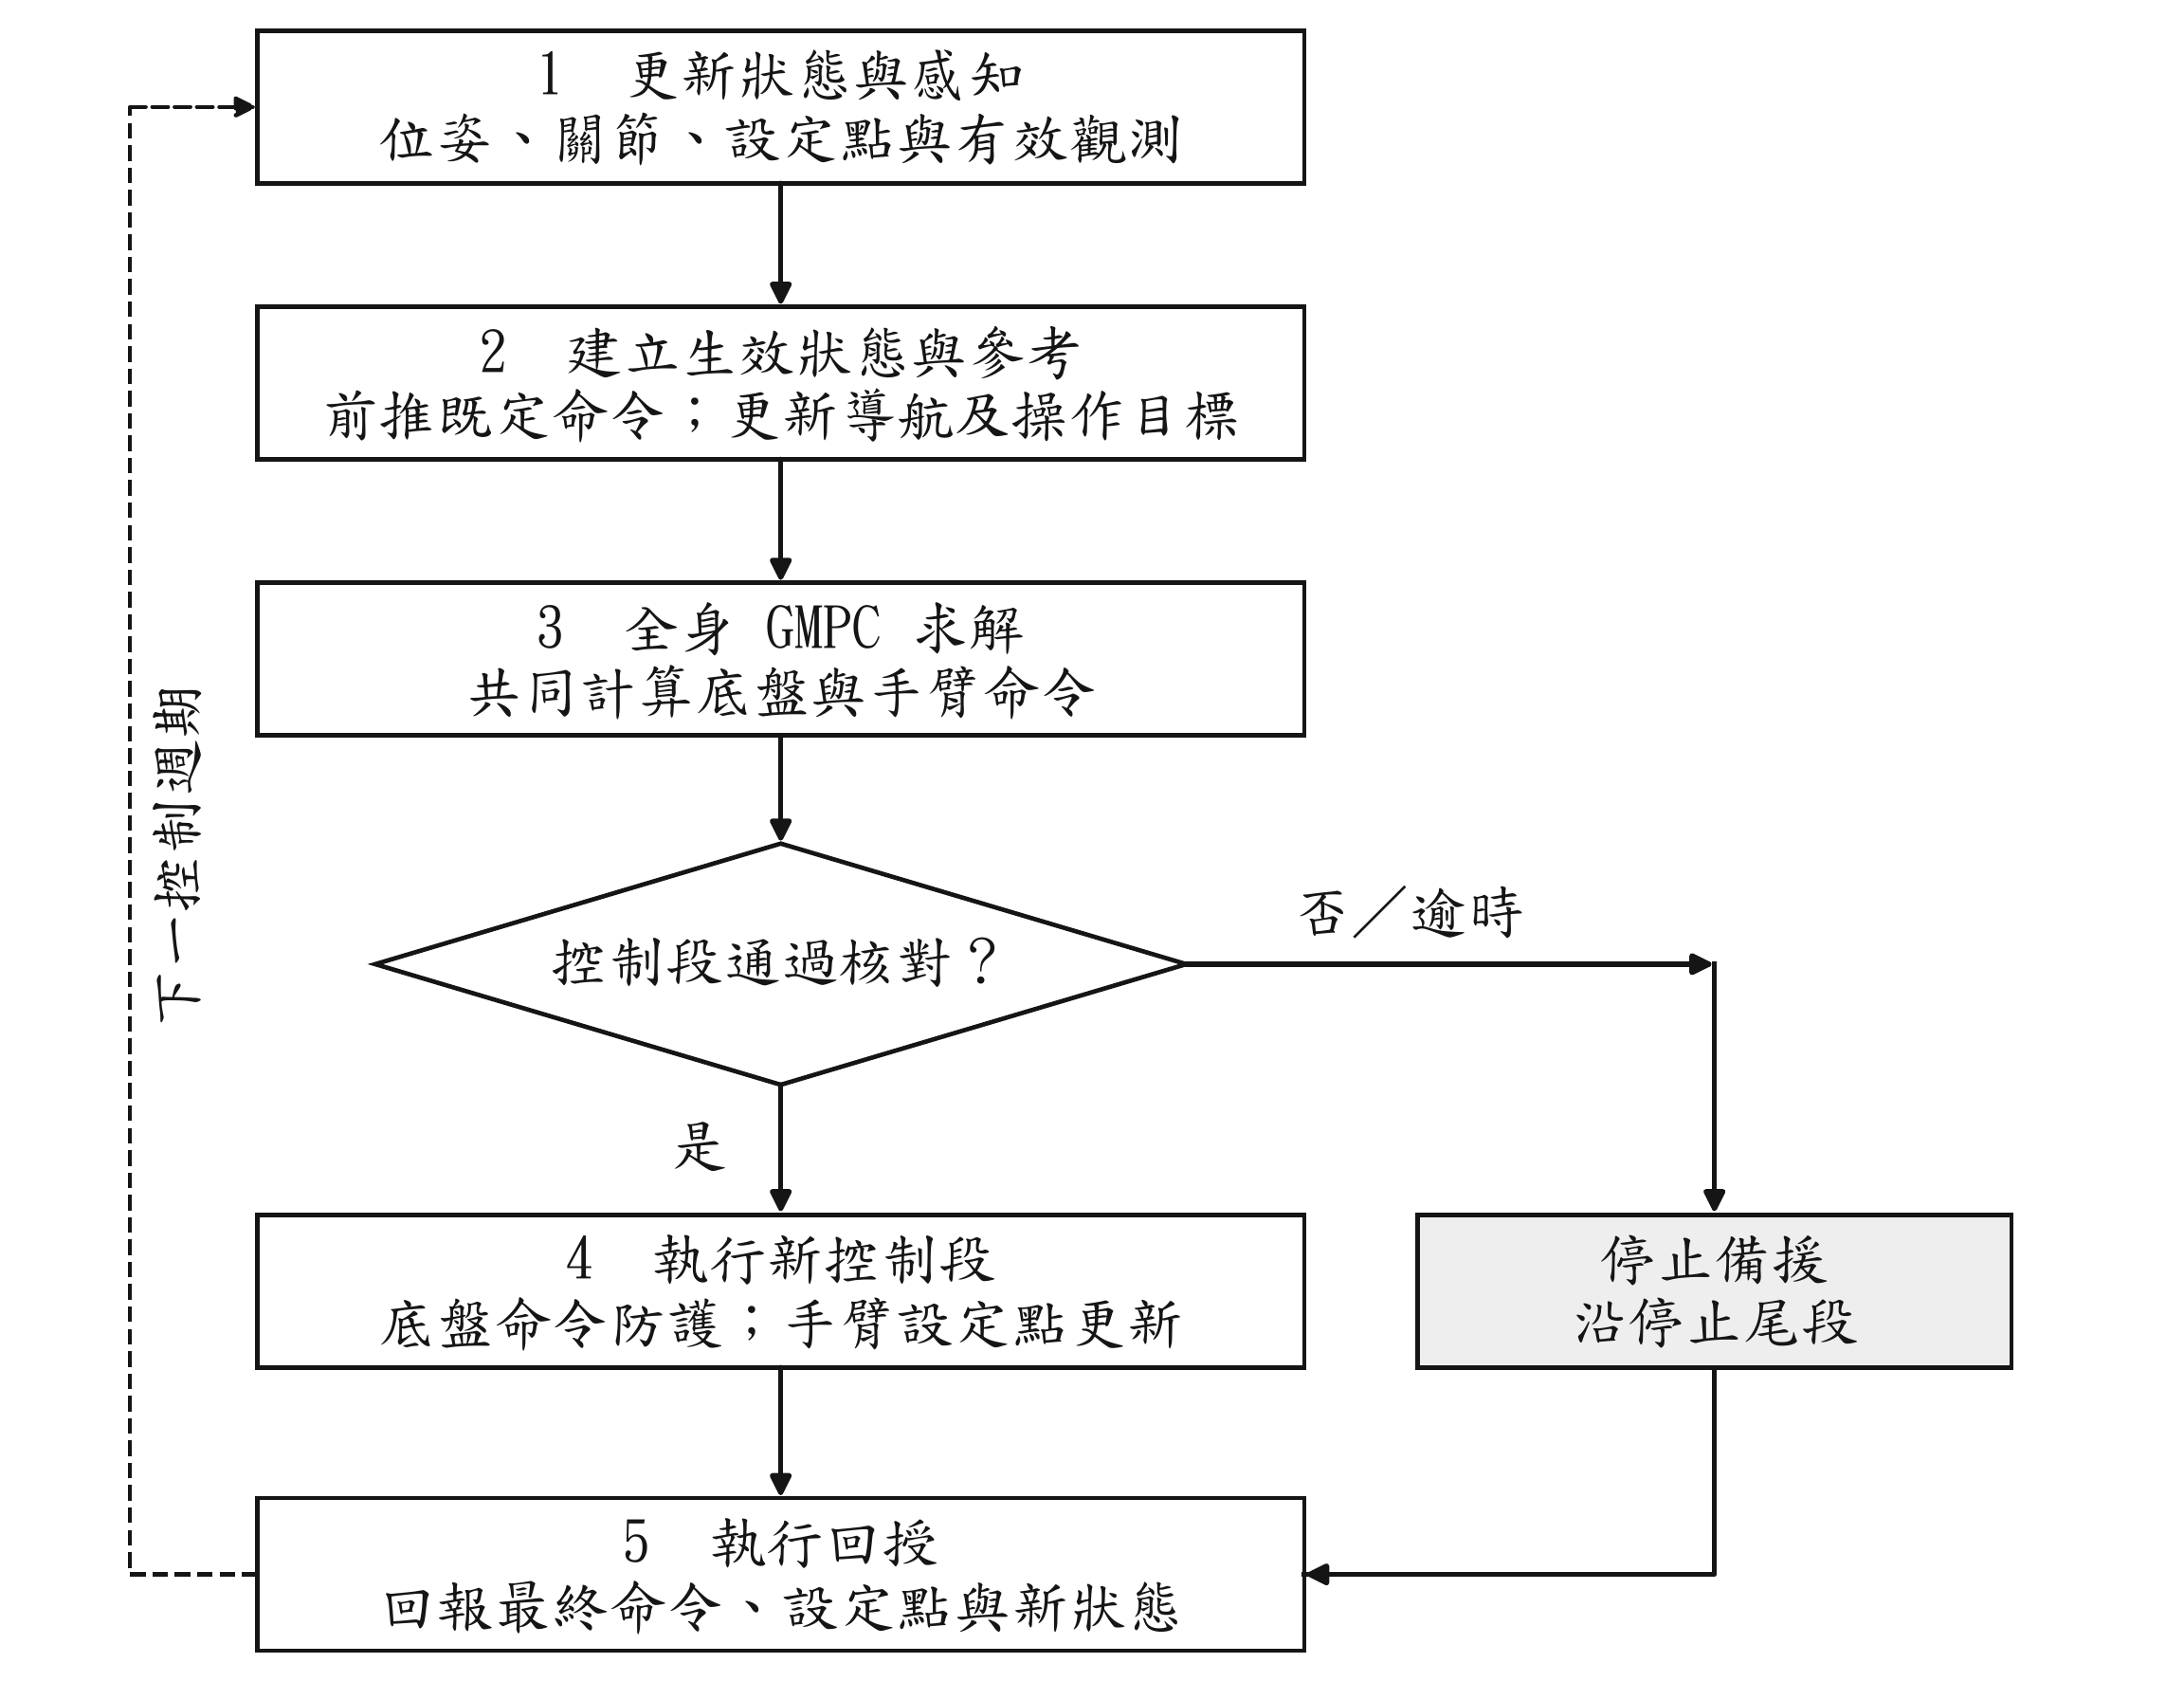
\includegraphics[width=0.82\linewidth,height=0.38\textheight,keepaspectratio]{figsrc/ch03/wholebody_control_workflow.png}
    \caption{全身預測控制之計算、命令核對與執行回授流程。}
    \label{fig:ch3_wholebody_control_workflow}

    \vspace{0.5\baselineskip}
\begin{algorithm}[H]
    \ifdefined\RawFloats\RawFloats\fi
    \fontsize{11pt}{13pt}\selectfont
    \setstretch{1.0}
    \setlength{\abovecaptionskip}{3pt}
    \setlength{\belowcaptionskip}{3pt}
    \hrule height 0.8pt\relax
    \caption{具命令承接與停止備援之全身預測控制}
    \label{alg:wholebody_predictive_control}
    \par\vspace{2pt}
    \hrule height 0.4pt\relax
    \vspace{4pt}
    \begin{algorithmic}[1]
        \Require State and sensor data, task state, navigation path,
                 scheduled commands, and model parameters
        \Ensure Applied commands, setpoints, task events, and stopping records
        \State Preserve the accepted segment and its stopping tail
        \While{the task is active or stopping is incomplete}
            \If{an update is due and the solver is available}
                \State Validate data and update enabled bias estimates
                \State Propagate scheduled commands to the activation time
                \State Update targets, references, and obstacle predictions
                \State Launch asynchronous QP solving and trajectory checks
            \EndIf
            \If{a candidate is ready and all checks pass}
                \State Submit a versioned packet with its activation step and stopping tail
            \EndIf
            \Statex \textbf{At every physics step:}
            \If{a valid packet reaches its activation step}
                \State Activate the new segment and its stopping tail
            \ElsIf{stopping is requested or the segment is nearly exhausted}
                \State Execute the applicable stopping tail; abort if necessary
            \EndIf
            \State Process base commands and integrate arm setpoints
            \State Report applied inputs, states, and task events
        \EndWhile
    \end{algorithmic}
    \par\vspace{4pt}
    \hrule height 0.8pt\relax
\end{algorithm}
    \end{minipage}
    \end{lrbox}
    % Scale down only when the complete box exceeds the page-height limit.
    \ifdim\dimexpr\ht\chThreeWorkflowAlgorithmBox+\dp\chThreeWorkflowAlgorithmBox\relax>0.98\textheight
        \resizebox*{!}{0.98\textheight}{\usebox{\chThreeWorkflowAlgorithmBox}}
    \else
        \usebox{\chThreeWorkflowAlgorithmBox}
    \fi
\end{figure}

第四章依模型預測、動態導航、協同操作及住宅整合任務，
說明實際配置、比較條件與驗證結果。
